\documentclass [twoside,openright,a4paper,11pt,french] {report}

    % Règles de typographie françaises
    \usepackage[francais]{babel}

    % Jeu de caractères UTF-8
    \usepackage[utf8]{inputenc}
    \usepackage[T1]{fontenc}

    % Fonte élégante
    \usepackage {mathpazo}
    \usepackage [scaled] {helvet}
    \usepackage {courier}

    % pour \EUR
    \usepackage {marvosym}

    \usepackage{emptypage}

    % Utilisation de tableaux
    \usepackage {tabularx}

    % Utilisation d'url
    \usepackage {url}
    \urlstyle {sf}

    % Utilisation d'images
    \usepackage{graphicx}
    \setkeys {Gin} {keepaspectratio}	% par défaut : conserver les proportions

    % Définition des marges
    \usepackage [margin=25mm, foot=15mm] {geometry}

    \parskip=2mm
    \parindent=0mm

    \pagestyle {plain}

\begin{document}

%%%%%%%%%%%%%%%%%%%%%%%%%%%%%%%%%%%%%%%%%%%%%%%%%%%%%%%%%%%%%%%%%%%%%%%%%%%%%%
% Page de garde
%%%%%%%%%%%%%%%%%%%%%%%%%%%%%%%%%%%%%%%%%%%%%%%%%%%%%%%%%%%%%%%%%%%%%%%%%%%%%%

\thispagestyle{empty}

\begin{center}
    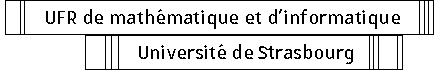
\includegraphics [width=10.1cm] {logo-ufr.pdf}       

    \vfill\vfill

    {
	\large
	\textsc {
	    Licencemaster 2 de Science, mention Informatique \\
	    spécialité Réseaux Informatiques et Systèmes Embarqués
	}
    }

    \bigskip\bigskip

    {\large Présenté par}

    \medskip

    % Identité de l'auteur
    {\large Jacques \textsc {Sélère}}

    % Contact mail ou téléphone   
    {\small \url{jselere@unistra.fr}}

    \vfill\vfill

    % Titre du stage
    {
	\huge
	\textsc {
	    Comment faire un bon \\
	    ~ \\
	    mémoire de stage ?
	}
    }

    \vfill\vfill

    {\large Encadré par}

    \medskip

    % Identité de l'encadrant
    {\large Jean \textsc {Breille}}

    % Contact mail ou téléphone
    {\small +33 (0) 3.68.85.98.76}

    \bigskip

    {\large Au sein de}

    \medskip

    % Structure d'accueil
    {
	\large
	\textsc {Société de propulsion aéroportée des escargots}
    }

    \vfill\vfill\vfill

    % Logo de votre structure d'accueil
    
\includegraphics [height=2.5cm] {logo-entreprise.pdf}       

\end{center}

% Page blanche au dos de la page de garde
\cleardoublepage

%%%%%%%%%%%%%%%%%%%%%%%%%%%%%%%%%%%%%%%%%%%%%%%%%%%%%%%%%%%%%%%%%%%%%%%%%%%%%%
% Table des matières
%%%%%%%%%%%%%%%%%%%%%%%%%%%%%%%%%%%%%%%%%%%%%%%%%%%%%%%%%%%%%%%%%%%%%%%%%%%%%%

{
    \parskip=0pt
    \tableofcontents
}

% Page blanche entre la table des matières et le texte
\cleardoublepage

%%%%%%%%%%%%%%%%%%%%%%%%%%%%%%%%%%%%%%%%%%%%%%%%%%%%%%%%%%%%%%%%%%%%%%%%%%%%%%
% Chapitre 1
%%%%%%%%%%%%%%%%%%%%%%%%%%%%%%%%%%%%%%%%%%%%%%%%%%%%%%%%%%%%%%%%%%%%%%%%%%%%%%

\chapter {Introduction}
    \label {chap:intro}

Le mémoire est un élément essentiel de votre stage : il a pour objet
d'exposer, le plus fidèlement possible, à la fois le périmètre du
stage (périmètres organisationel et/ou technique) et votre contribution.

Votre mémoire sera lu par un «~rapporteur~», c'est-à-dire un
enseignant de l'équipe pédagogique (donc une personne ayant des
compétences dans votre discipline), dont la mission est d'évaluer votre
mémoire pour comprendre le contexte dans lequel vous avez évolué,
et votre contribution (réalisation technique, travail scientifique ou
autre) ainsi que son adéquation vis-à-vis de la formation.

Ce document a pour but de rappeler les éléments attendus par le
rapporteur pour évaluer votre travail. Il est de votre intérêt de
fournir tous ces éléments.


%%%%%%%%%%%%%%%%%%%%%%%%%%%%%%%%%%%%%%%%%%%%%%%%%%%%%%%%%%%%%%%%%%%%%%%%%%%%%%
% Chapitre 2 : le plan
%%%%%%%%%%%%%%%%%%%%%%%%%%%%%%%%%%%%%%%%%%%%%%%%%%%%%%%%%%%%%%%%%%%%%%%%%%%%%%

\chapter {Le plan}
    \label {chap:plan}

Votre mémoire doit être bien structuré, c'est-à-dire présenter une
progression logique et apparente. Le plan est de votre responsabilité,
mais il doit comporter des chapitres relativement équilibrés (en taille)
et contenir les éléments décrits ci-après (un élément n'est pas
forcément un chapitre en soi). Les enchaînements entre les chapitres
et les sections doivent être compréhensibles.

N'omettez pas la table des matières, et numérotez vos chapitres et
vos sections (1, 1.1, 1.1.1, etc.), cela aide à se repérer.

\section {L'organisme d'accueil}

L'exercice consiste à présenter une description de votre contexte
organisationnel : votre rapporteur ne connaît à priori pas
l'organisme d'accueil, donc vous devez le présenter à travers sa
branche d'activité, ses chiffres caractéristiques. De plus, vous
devez présenter votre place dans l'organisme : vous devez suivre une
description en «~entonnoir~» (voir figure~\ref {fig:entonnoir}),
c'est-à-dire partir de l'organisme dans son ensemble pour arriver
jusqu'à votre place en tant que stagiaire. Un organigramme peut aider
à comprendre votre place dans l'organisme ou le service concerné.

\begin {figure} [htbp]
    \begin {center}
	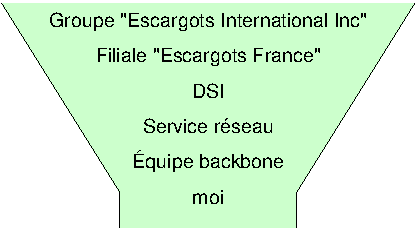
\includegraphics [width=.4\textwidth] {entonnoir.pdf}
    \end {center}
    \label {fig:entonnoir}
    \caption {Description de l'organisme : du plus large jusqu'à vous.}
\end {figure}

La figure~\ref {fig:entonnoir} présente la démarche : évoquer le
groupe au plus haut niveau (ses activités, son chiffre d'affaires, sa
présence dans le monde, le nombre d'employés, etc.), puis présenter
la filiale française et ainsi de suite jusqu'à arriver à l'équipe
dans laquelle vous vous situez (en précisant ses missions, le nombre
de personnes, etc.) et votre place dans cette équipe.

Évitez de recopier un site Web : cela se voit et ça énerve souvent
le rapporteur. Rédigez un texte avec vos propres mots : même s'il y a
des maladresses, cela passera beaucoup mieux.

Notez que la présentation de la structure d'accueil est obligatoire,
même si vous savez que cette structure est bien connue de votre
rapporteur (par exemple pour un stage réalisé dans le laboratoire
ICube). L'exercice imposé est de présenter cette structure, et tous
les stagiaires sont évalués sur ce critère, sans exception.

\section {La mission}
    \label {sec:mission}

En tant que stagiaire, vous avez une mission définie correspondant à
la durée de votre stage. Décrivez cette mission, en la mettant en
perspective par rapport aux besoins de l'organisme. De plus, donnez
les contraintes particulières (financières, technique ou autres)
ainsi que les objectifs à atteindre, qui permettront d'évaluer ou
non la réussite du projet.

\section {Le contexte}

Le contexte technique ou organisationnel doit être présenté.
Rappelez-vous que votre rapporteur a une bonne maîtrise des concepts
techniques, mais qu'il n'a pas connaissance des contraintes particulières
liées à votre organisme d'accueil ou à son métier.

N'abusez pas du contexte : vous devez présenter le minimum pour permettre
au rapporteur de comprendre les contraintes spécifiques de votre stage
et votre contribution. Pas plus.


\section {Votre contribution}

C'est la principale partie de votre mémoire : vous devez présenter votre
contribution (réalisation logicielle, système informatique, état de
l'art, méthode, algorithme, évaluation, etc.) de façon synthétique,
sans sombrer dans les détails techniques mais en n'éludant pas les
points concrets qui permettent au rapporteur d'avoir une vision la plus
précise possible de ce que vous avez mis en {\oe}uvre.

Soyez précis et factuel : technologies, algorithmes ou méthodes
employés, éléments quantitatifs permettant d'apprécier l'envergure
du projet, comparatifs réalisés, etc. Si vous avez travaillé en
coopération avec d'autres personnes (votre maître de stage, d'autres
personnes ou stagiaires), indiquez avec précision votre rôle et vos
réalisations.

La méthodologie avec laquelle vous procédez est l'un des principaux
critères d'évaluation de votre travail : les problèmes doivent
être analysés, les choix effectués (ou auxquels vous avez pris part)
doivent être explicités et justifiés.

\section {Votre bilan}

Le stage complète votre formation : vous devez prendre du recul pour
mettre en rapport votre stage avec les compétences aquises pendant
votre formation, ainsi que présenter les compétences complémentaires
(techniques et/ou personnelles) que vous avez aquises durant le stage.

Le bilan doit montrer votre recul par rapport au stage : vous avez
le droit (voire le devoir) de jeter un regard critique sur votre
comportement, sur votre démarche, sur votre réalisation ou même sur
le contexte ou l'organisme d'accueil.


%%%%%%%%%%%%%%%%%%%%%%%%%%%%%%%%%%%%%%%%%%%%%%%%%%%%%%%%%%%%%%%%%%%%%%%%%%%%%%
% Chapitre 3
%%%%%%%%%%%%%%%%%%%%%%%%%%%%%%%%%%%%%%%%%%%%%%%%%%%%%%%%%%%%%%%%%%%%%%%%%%%%%%

\chapter {La forme}
    \label {chap:contexte}

Un bon mémoire allie un fond de qualité et une forme parfaite. Quelques
règles de bon sens s'appliquent.

\section {Typographie}

La rédaction de textes français obéit à des règles précises en
Français : cela s'appelle la «~typographie~» \cite{andre1990} et il
est intéressant de s'en imprégner pour éviter des erreurs grossières
et donner à votre document un aspect de qualité.

\section {L'orthographe et la grammaire}

L'orthographe et la grammaire sont des prérequis indispensables pour
la rédaction du mémoire. Si vous n'êtes pas sûr de vous, faites-vous
relire par un tiers. C'est dommage de perdre des points sur ce critère.

\section {Numérotez}

Numérotez tout ce qui peut l'être : pages, chapitres, sections, figures,
tables, bibliographie. Laissez à votre logiciel le soin de numéroter
automatiquement, il le fera mieux que vous «~manuellement~». Utilisez
des références si vous devez mettre en relation plusieurs éléments
de votre discours (exemple fictif : voir la figure~\ref {fig:entonnoir}
page~\pageref {fig:entonnoir}, ou encore le chapitre~\ref {chap:plan}
et plus spécifiquement la section~\ref {sec:mission}, page~\pageref
{sec:mission}).


\section {Les illustrations}

Un petit dessin valant mieux qu'un grand discours, les schémas de
principe sont souvent appréciés par le rapporteur, qui ne connaissent
pas votre environnement. Quelques règles cependant sont à respecter :

\begin {itemize}
    \item numérotez et légendez vos figures (voir figure~\ref
	{fig:entonnoir}, page~\pageref {fig:entonnoir}, par exemple)~;
    \item référencez vos figures : une figure non référencée dans le
	texte ne sert à rien~;
    \item expliquez vos figures dans le texte : si une figure n'a pas
	besoin d'explication, cela signifie qu'elle est sans doute trop
	simple et n'a donc pas besoin de figurer dans votre mémoire~;
    \item citez la provenance de vos figures, si elles ne sont pas de
	vous : il est parfaitement admis d'utiliser des figures
	réalisées par d'autres, si vous citez la provenance~;
    \item les logos de logiciels ou de produits sont à bannir~: ils
	n'apportent rien à la compréhension de votre mémoire et ne font
	que prendre de la place inutile que vous pourriez utiliser pour
	mieux présenter votre contribution~;
    \item vérifiez que vos figures sont lisibles lorsque vous imprimez
	votre mémoire.
\end {itemize}

Les copies d'écran n'apportent généralement pas grand-chose~: elles
contiennent trop d'informations inutiles et sont peu lisibles. De plus,
le message véhiculé est souvent très succint, voire trop léger. Un
fichier de configuration, une commande ou son résultat doivent être
présentés, si c'est vraiment nécessaire, comme du texte et non comme
une copie d'écran.

\section {La bibliographie}

La bibliographie constitue une partie importante de votre mémoire.
Elle constitue un critère de qualité du travail (avez-vous trouvé les
bonnes sources ? les documents sur lesquels vous vous appuyez sont-ils
sérieux ?). Vous devez indiquer les documents~:

\begin {itemize}
    \item de référence que vous avez consultés dans votre recherche,
	pour vous familiariser avec votre sujet ou pour apprendre
	des techniques particulières~;
    \item que vous avez consultés pour effectuer vos choix ou mettre
	en {\oe}uvre un dispositif logiciel ou autre~;
    \item qui permettent au lecteur d'en savoir plus sur tel ou tel
	point de votre mémoire que vous ne pouvez davantage développer.
\end {itemize}

La bibliographie~\cite {savoirs2010} vient en annexe, elle doit donner
tous les renseignements nécessaires pour permettre au lecteur de
retrouver les documents concernés~: auteur, titre du document ou de
l'ouvrage, éditeur, année de publication, URL si nécessaire, date de
consultation pour un site Web, etc.

Chaque document dans la bibliographie comporte une référence
(un numéro, une abbréviation ou autre), que vous pouvez citer dans le
texte.

%%%%%%%%%%%%%%%%%%%%%%%%%%%%%%%%%%%%%%%%%%%%%%%%%%%%%%%%%%%%%%%%%%%%%%%%%%%%%%
% Conclusion
%%%%%%%%%%%%%%%%%%%%%%%%%%%%%%%%%%%%%%%%%%%%%%%%%%%%%%%%%%%%%%%%%%%%%%%%%%%%%%

\chapter {Conclusion}
    \label {chap:conc}

Il est maintenant temps de rédiger votre mémoire. Puissent ces quelques
conseils vous guider afin de vous aider à présenter le mieux possible
tout le travail que vous avez effectué durant votre stage !


%%%%%%%%%%%%%%%%%%%%%%%%%%%%%%%%%%%%%%%%%%%%%%%%%%%%%%%%%%%%%%%%%%%%%%%%%%%%%%
% Bibliographie
%%%%%%%%%%%%%%%%%%%%%%%%%%%%%%%%%%%%%%%%%%%%%%%%%%%%%%%%%%%%%%%%%%%%%%%%%%%%%%

\cleardoublepage
\bibliographystyle{plain}
\bibliography{rapport}

\end{document}
